% Final Paper
% Digital Multimedia Coding and Processing
% 5/10/10

\documentclass[10pt,twocolumn,twoside]{IEEEtran}

\usepackage[centertags]{amsmath}
\usepackage{graphicx, latexsym, amsfonts, amssymb, epsf, cont}

\def\BibTeX{{\rm B\kern-.05em{\sc i\kern-.025em b}\kern-.08em T\kern-.1667em\lower.7ex\hbox{E}\kern-.125emX}}

\newtheorem{theorem}{Theorem}
\renewcommand{\O}[1]{\textit{O}(\ensuremath{#1})}

\begin{document}

% Title
\title{A Parallel Image and Video Processing Application}
\author{H. Parker Shelton, Adam Feinstein
\thanks{The authors are with the Departments of Computer Science and Electrical and Computer Engineering, The Johns Hopkins University, Baltimore, MD 21218.
Email: \{parker.shelton, afeinst1\}@jhu.edu.}}

\maketitle
\vskip -20pt

\begin{abstract}
We built a go-fast image and video editor.
\end{abstract}

\section{Introduction}
\PARstart{M}{ultimedia}

\section{GPUs and CUDA}
Dedicated graphical processing units (GPUs) have become more prevalent in modern computers. This specialized hardware differs from traditional CPUs in that it is designed to preform parallel arithmetic computations. While the GPU is almost always used for 3D intensive applications, such as gaming, it is rarely tapped into for general computing tasks. In order to use this computational power in a general computing environment, NVIDIA has developed Compute Unified Device Architecture (CUDA). CUDA-enabled code can be executed on all of NVIDIA's modern GPUs (those developed in the past three years). These include the consumer GeForce series, the professional Quadro and Tesla cards, and even the ION series of GPUs, found in netbooks and small form factor media centers.
	
CUDA allows the programmer to allocate the GPU's multiprocessors in order to run parallel computations. A GPU's hardware is divided into blocks and threads. Each block contains a fixed number of threads, and each thread is capable of running one calculation. Each active thread must run the same calculation, but each thread may preform the calculation on a different value in memory. A diagram of the task allocation can be seen in Figure \ref{fig:cudaBlocks}.

\begin{figure}[h]
\begin{center}
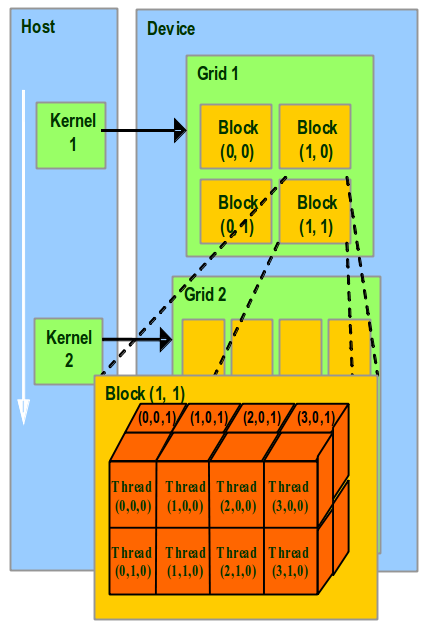
\includegraphics[width=0.35\textwidth]{cudaBlocks.png}
\caption{Task allocation between grids, blocks, and threads in a GPU}
\label{fig:cudaBlocks}
\end{center}
\end{figure}
	
Memory is not shared by the GPU and the CPU. Memory must be copied from the host (CPU) to the device (GPU) when a calculation must be preformed. This memory transfer runs in \O{n} time. Because memory must be copied, certain operations such as matrix subtraction are not well suited to be parallelized. A matrix subtraction on the GPU would take \O{n} time for the memory transfer and \O{n/threads} time for the operation, whereas whereas the same operation on the CPU will take \O{n} time.

Memory on the GPU is divided into global memory, which is accessible from each thread in each block, shared memory, which is accessible from each thread in a given block, but not threads in other blocks, and register memory, which is only accessible from a single thread. The memory diagram for a GPU is shown in Figure \ref{fig:cudaMem}. Registers are accessed faster than shared memory, which is in turn accessed faster than global memory. When data is moved from the CPU to the GPU, it is placed in global memory.

\begin{figure}[h]
\begin{center}
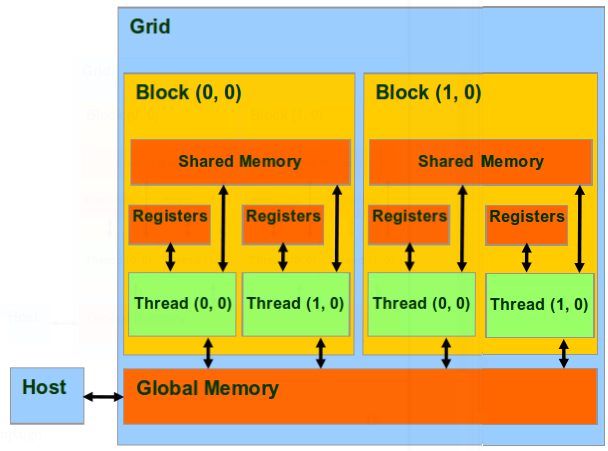
\includegraphics[width=0.35\textwidth]{cudaMem.png}
\caption{GPU memory heirarchy}
\label{fig:cudaMem}
\end{center}
\end{figure}

\section{User Interface}
A significant portion of the development of the editor was spent designing and implementing a graphical user interface (GUI) to display the result of the editing operations performed. The user interface was written in C++ using a cross-platform framework called Qt, available from Nokia under a LGPL open-source license. The use of Qt allowed for rapid GUI development and created a beneficial abstraction of GUI commands into image editing function calls. 

As Qt also contains a multimedia framework, its use simplified the extension of the program to standard image formats; the QImage class provided support for reading .bmp, .gif, .jpg, .png, .pgm, and .tif files from disk, as well as writing .bmp, .jpg, .png, .tif with an optional quality setting. In addition to the standard image formats provided by QImage, custom image (.ppc) and video (.pvc) codecs were created and encoders and decoders implemented. These will be discussed further in a later section.

The GUI is arranged to display the original image on the left and the modified image on the right. The scale of the images can be changed using zoom functions, and the modified image can be reset to the original image without requiring reopening, and thus decoding, the file from disk. This functionality was provided in lieu of undo/redo functionality, which would require either a large amount of memory to be allocated or the creation of inverse functions for all implemented functionality. Videos can be played using a control bar at the bottom that also allows for frame by frame inspection.

Compression is implemented so as to display a new dialog containing both the modified media and the compressed version. This allows for side-by-side comparison of the compression quality achieved as well as comparison among multiple compression levels. The peak signal-to-noise ratio (PSNR) is also reported as a measure of the compression quality chosen. 

\section{Image Editing}
Several common image editing operations were explored and then implemented in the editor. These were then further extended to video editing by applying them to each frame sequentially. Each operation implemented is discussed in detail below.

\subsection{Grayscale}
Because the image was stored internally in ARGB format, the conversion to grayscale requires application of the luminance formula to each pixel: \begin{equation*}luminance = 0.3*red + 0.59*green + 0.11*blue \end{equation*}
This is in contrast to an image in YCrCb format, where the color space would simply be thrown away. The luminance result was then clamped to fit into an 8-bit unsigned char (0 $\leq$ value $\leq$ 255) and assigned to all of the red, green, and blue color values. All values resulting from color calculations in all future editing operations can be assumed to be clamped to the same range before being assigned to the resulting image. 

\subsection{Brightness}
Increasing the brightness of an image can be achieved by scaling each of the RGB values by a specified factor. This adjusts the luminance of the entire image.

\subsection{Contrast}
Contrast is a measure of the distance of each pixel from the average luminosity. In order to increase contrast,  a linear combination of the average luminosity and the RGB values are taken:
\begin{equation*} red = (1 - factor)*average\_lum + (factor)*red \end{equation*}

\subsection{Saturation}
In contrast to contrast, increasing saturation requires scaling the RGB values of a pixel away from its luminosity, rather than the global average luminosity. The formula appears the same as for contrast, with $average\_lum$ replaced with $lum$.

\subsection{Crop}
Cropping was implemented to remove unwanted portions or highlight desired portions of an image. The function takes four parameters defining the top-left and bottom-right corners of the desired sub-image.

\subsection{Rotation}
Rotation was implemented using both Gaussian sampling and nearest-neighbor sampling of the original image in order to determine pixel color values in the rotated image. If the image rotation is a multiple of 90$^\circ$, nearest-neighbor sampling is used to generate a one-to-one matching, while Gaussian rotation is used otherwise. The Gaussian used was defined with variance 0.6 and radius 4 pixels. 

\subsection{Scale}
Scaling was also implemented using Gaussian sampling, also with variance 0.6, but with a radius that linearly depends on the scaling factor to compensate for the enlarged (or shrunken) size of the image.

\subsection{Blur}
Blurring was performed using a 3x3 convolution filter that weights the original pixel heavily, but allows for contributions from neighboring pixels:
\begin{equation*}
mask[3][3] = \left\{ \left\{\frac{1}{16}, \frac{2}{16}, \frac{1}{16}\right\}, \left\{\frac{2}{16}, \frac{4}{16}, \frac{2}{16}\right\}, \left\{\frac{1}{16}, \frac{2}{16}, \frac{1}{16}\right\} \right\}
\end{equation*}

\subsection{Edge Detection}
Edge detection was similarly implemented as a 3x3 matrix convolution, but with a mask that highlights pixels with colors sufficiently different from its neighbors:
\begin{equation*}
mask[3][3] = \left\{ \left\{-1, -1, -1\right\}, \left\{-1, 8, -1\right\}, \left\{-1, -1, -1\right\} \right\}
\end{equation*}

\section{Compression}
The two compression algorithms that were implemented both sequentially and in parallel were the biorthogonal 9/7 discrete wavelet transform (DWT) with a dead-zone quantizer for images and a closed-loop DPCM quantizer with motion estimation for videos.

\subsection{DWT? FWT? Compression}
	
The particular implementation of the DWT that was used was the lifting implementation. This implementation is the same one used in the JPEG2000 standard. The transform works on an array of real values. The values are filtered into low and high frequency sub-bands, which are each downsampled by a factor of two. The high pass sub-band is retained in the odd indices of the array, while the low pass sub-band is retained in the even indices of the array. The inverse transform is preformed using the same computational structure, but with inverse filters.

A sketch of the algorithm for image transformation is as follows. First, the image is transferred into GPU memory. The different color components must be transformed separately, so the ARGB image data is rearranged such that all the red, blue, and green values are in continuous memory. This is done in one parallel step, where each thread moves one color value, and is not done in-place. Each row of each continuous color region is then transformed in parallel. Due to the iterative nature of the FWT, the algorithm cannot be preformed in one step. Once each row is transformed, each continuous color region is transposed separately. The FWT is then applied to each row (previously column) of each continuous color region in parallel. This completes the one level 2D FWT. Another transpose, FWT, transpose, and FWT may be applied to perform the two level 2D FWT.

The inverse transform is simply the same process in reverse using the iFWT instead of the FWT, and rearranging the continuous color regions into 32 bit 0xffRRGGBB format.

\subsection{Video Compression}
A closed-loop DPCM quantizer with motion estimation was implemented for video compression. A sketch of the algorithm is as follows. For the first frame, the previous frame is set to all zeros. The encoded previous frame is subtracted from the current frame, $d[n]$, which is then quantized and inverse quantized, $\hat{d}[n]$. This value is summed with the encoded previous frame, $\hat{x}[n-1]$ and set as the new encoded previous frame for the next iteration, $\hat{x}[n]$. Motion vectors are then found for each 8x8 block which minimize the matrix $x[n]$ - $\hat{x}[n-1]$ + [motion vectors], and the quantized result along with the motion vectors are sent to the communication channel for encoding.

Decoding is simpler than encoding and involves simply summing the previous decoded frame, $\hat{x}[n-1]$, shifted by the motion vectors, with the inverse quantized incoming frame, $\hat{d}[n]$.

The parallelization comes into play with the search for optimal motion vectors. As previously stated, simple operations such as matrix addition or subtraction do not offer significant speedup when preformed on the GPU. An exhaustive search for motion vectors lends itself well to parallelization, however. Each block on the GPU is assigned one 8x8 block of pixels from the frame and the previous 8x8 block of pixels out of the frame !!! NOT SURE THIS IS PHRASED WELL !!!, and each thread within that block calculates one potential motion vector and the resulting sum of the absolute value of the difference between blocks. From this pool of all motion vectors, a parallel reduction is preformed, reducing the time to find the minimum value in an array from \O{n} in a serial implementation to \O{log(n)} in parallel. The first iteration of the reduction compares n/2 sets of 2 elements, and returns the smallest of each. The next iteration then compares n/4 sets of 2 elements, and returns the smallest of each. This continues until the smallest element is found. In this case, the motion vector with the smallest difference is found and returned.

Sample code which came with the CUDA SDK was modified and used for both the reduction and the transpose. A second set of non-parallelized algorithms are also supplied to compare with GPU accelerated algorithms, and for users who do not have a compatible GPU.

\section{Theorem}
\section{Performance Metrics}
\subsection{Coding Gain}
\section{Conclusion}

%\nocite{*}
\bibliographystyle{IEEEbib}
\bibliography{Multimedia}

\end{document}